\documentclass{beamer}
\usepackage{ctex}
\usepackage[utf8]{inputenc}
\usepackage{graphicx}
\usepackage{amsmath}
\usepackage{amssymb}
\usepackage{booktabs}
\usepackage{hyperref}
\usepackage{subcaption}
\usepackage{multicol}
\usepackage{listings}
\usepackage{multirow}
\usepackage{tabularx}


\usetheme{Madrid}
\usecolortheme{seahorse}

% 自定义块颜色
\setbeamercolor{block title}{bg=blue!30,fg=black}
\setbeamercolor{block body}{bg=blue!10,fg=black}
\setbeamercolor{alertblock title}{bg=red!50,fg=black}
\setbeamercolor{alertblock body}{bg=red!20,fg=black}

% 开启图表编号
\setbeamertemplate{caption}[numbered]

% ...existing code (theme settings, etc.)...

\title{\textbf{周报——向嘉豪(2024年12月24日)}}
\author{向嘉豪}
\institute{衡阳师范学院}
\date{2024年12月24日}

\begin{document}

\begin{frame}
    \titlepage
\end{frame}

\begin{frame}
    \frametitle{本周主要工作}
    \begin{block}{}
        \begin{itemize}
            \item 第二篇投稿
            \item 第三篇论文背调
        \end{itemize} 
    \end{block}
\end{frame}


\section{第二篇投稿}

\begin{frame}
    \frametitle{第二篇投稿}
    \begin{block}{}
        在准备投稿的过程中,研究了\textit{Computer}期刊的选题方向与投稿要求,并完成了针对最合适Topic的初步匹配。由于个人Biography信息不全导致稿件被退回,我们已补充完成该部分并再次提交,以期进入下一轮审查。
    \end{block}
\end{frame}

\section{第三篇论文背调}

\begin{frame}
    \frametitle{第三篇论文背调}
    \begin{block}{}
        在第三篇论文的背景调研中,我们考察了安全性、性能与成本三者间的关联,并针对不同安全等级与性能需求分析了软硬件加速方案。结论显示:若在高度安全的同时追求更高性能,则对应硬件加速;若严格控制成本,则性能相对较低,多采用纯软件实现。针对中等成本与中等性能,软硬件结合能够在绿色、蓝色区域之外形成平衡(红色区域)。
    \end{block}
    \begin{figure}[h]
        \centering
        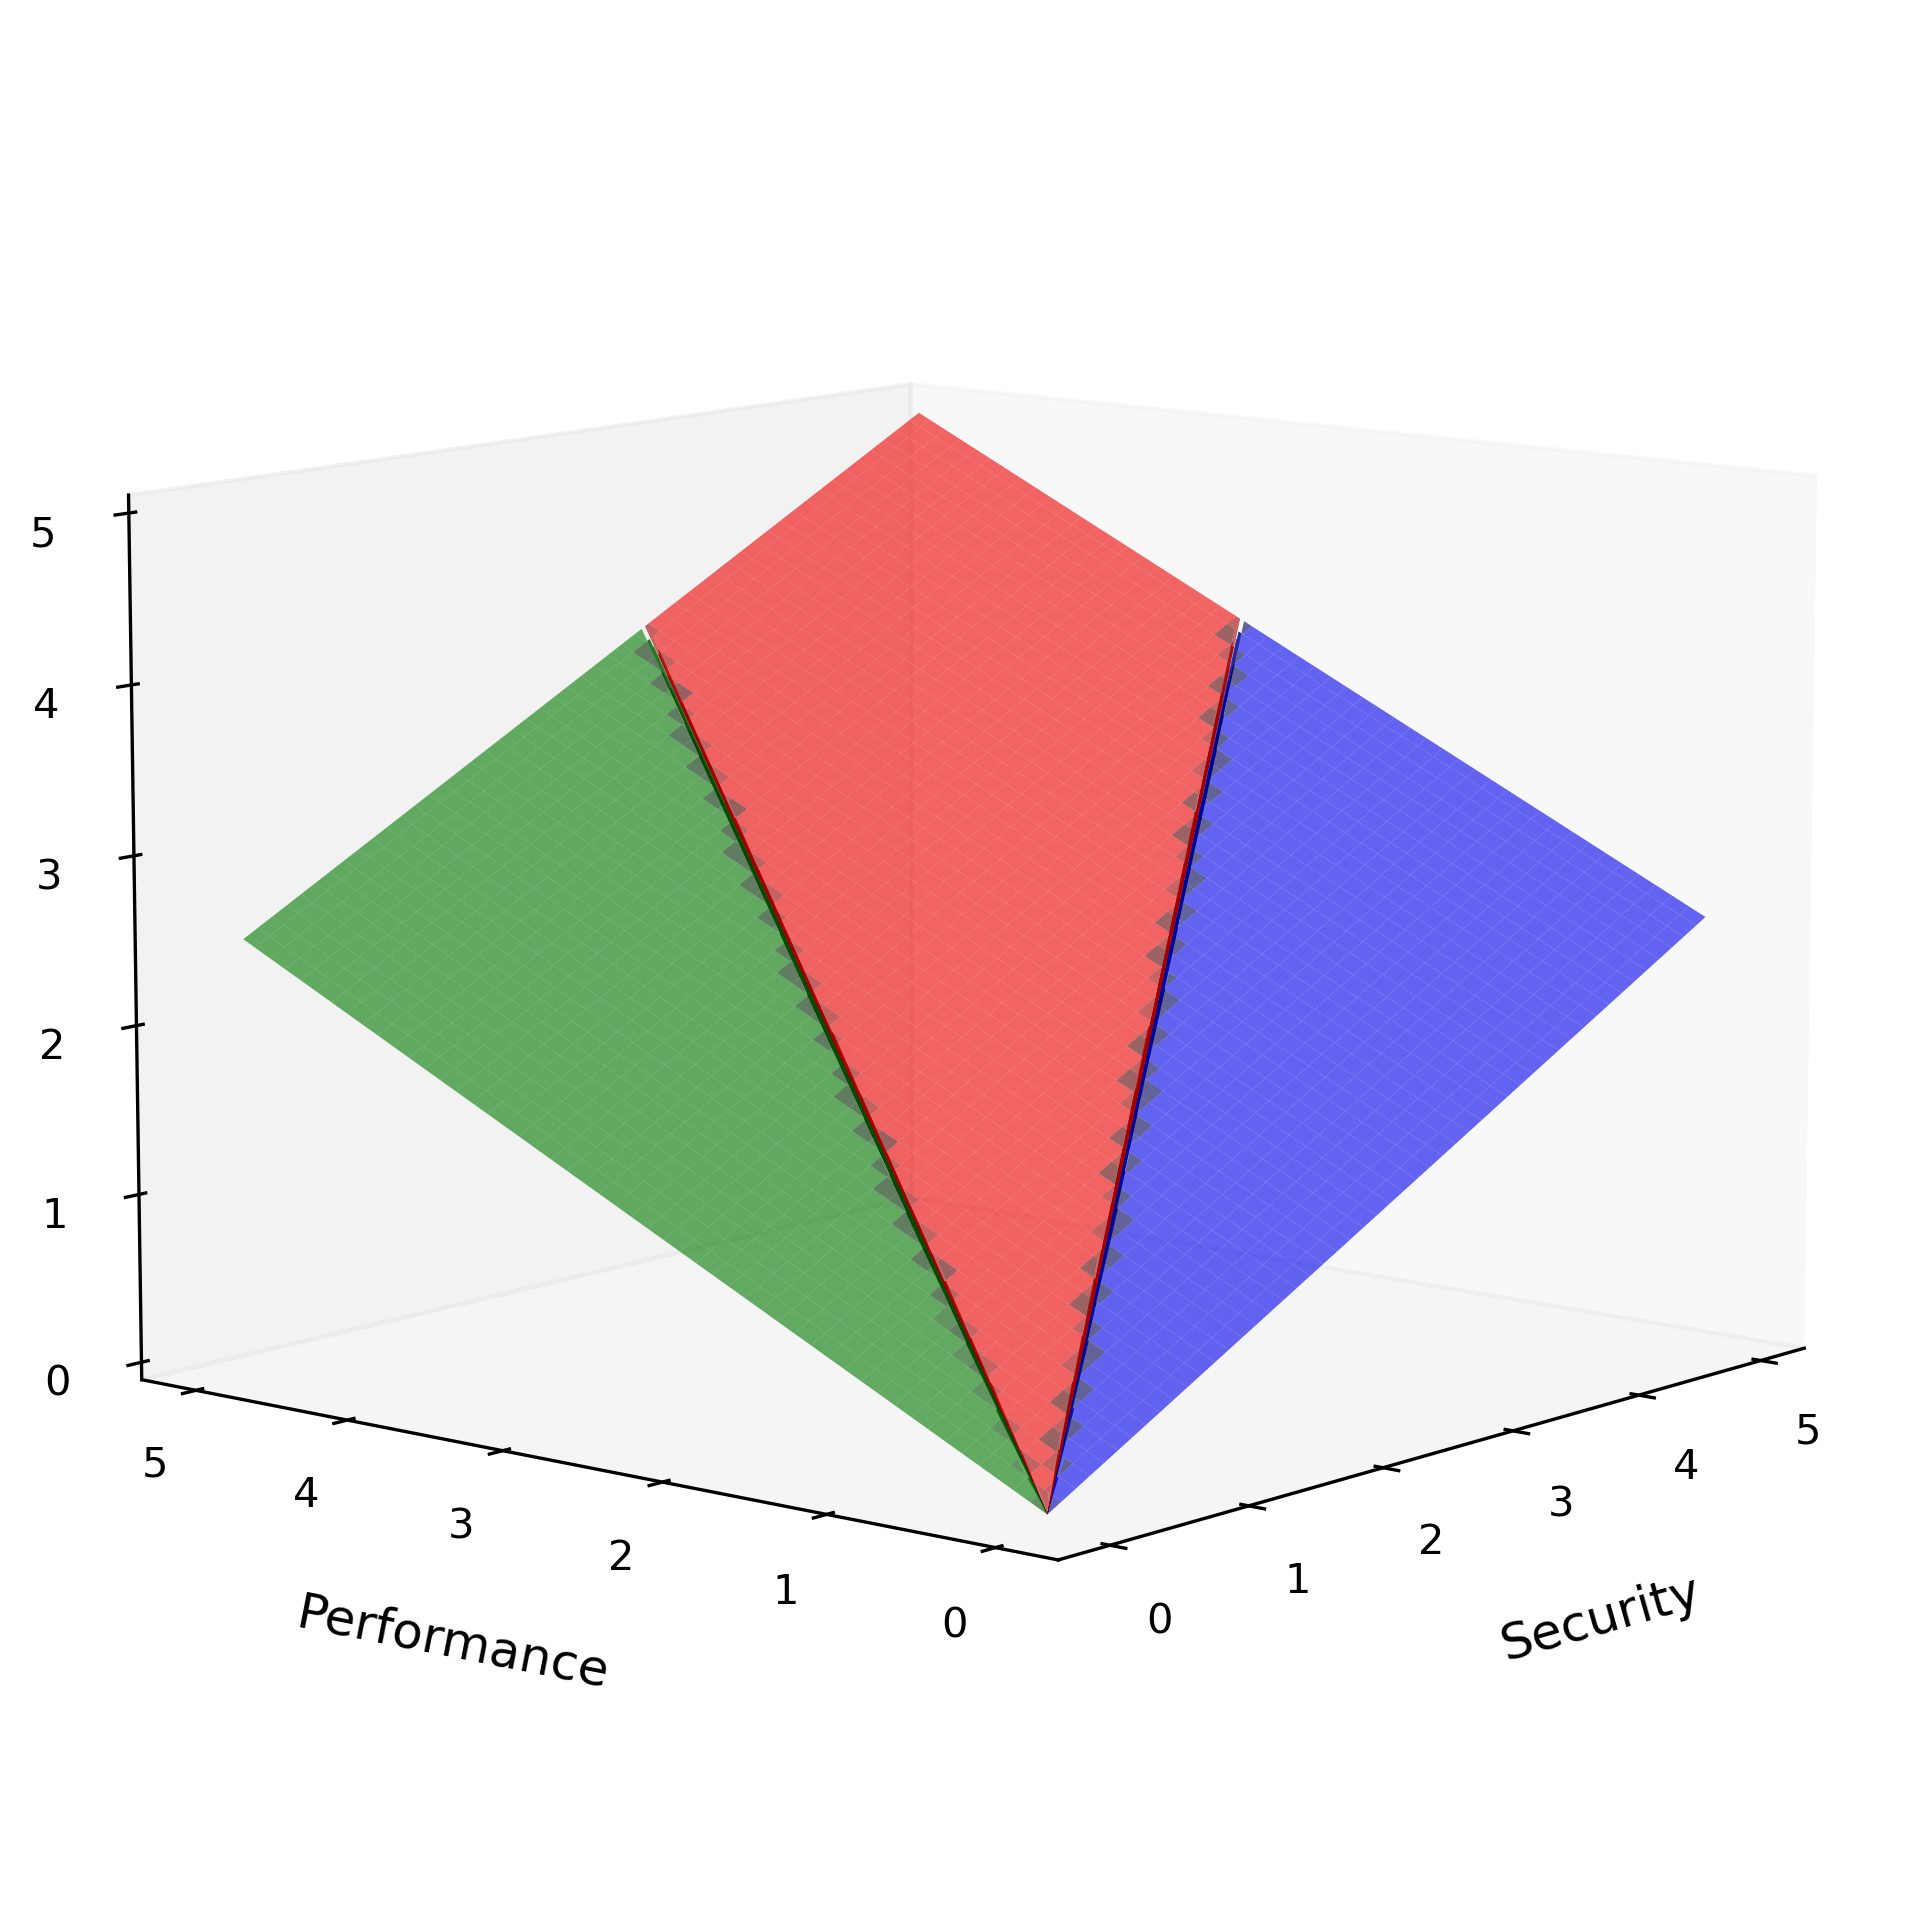
\includegraphics[width=0.35\textwidth]{./fig/SPC_relation.png}
        \caption{安全性、性能和成本的关系}
    \end{figure}
\end{frame}

\begin{frame}[fragile]
    \frametitle{Related Work: GPU-Based Cipher Implementations (Part I)}

       \begin{table}[h]
        \centering
        \resizebox{.9\textwidth}{!}{
        \begin{tabular}{p{6cm} p{1.5cm} p{4.5cm}}
            \toprule
            \textbf{Paper Name} & \textbf{Year} & \textbf{Publication} \\
            \midrule
            Speed Record of AES-CTR and AES-ECB Bit-Sliced Implementation on GPUs & 2024 & IEEE EMBEDDED SYSTEMS LETTERS \\
            Optimized GPU Implementation and Performance Analysis of HC Series of Stream Ciphers & 2012 & Information Security and Cryptology \\
            High Throughput Implementation of Post-quantum Key Encapsulation and Decapsulation on GPU for IoT Applications & 2021 & IEEE Transactions on Services Computing \\
            Fast AES Implementation–A High-Throughput Bitsliced Approach & 2019 & IEEE Transactions on Parallel and Distributed Systems \\
            \bottomrule
        \end{tabular}
        }
        \caption{Summary of GPU-based cipher implementations (Part I)}
    \end{table}
\end{frame}

\begin{frame}[fragile]
    \frametitle{Related Work: GPU-Based Cipher Implementations (Part II)}

       \begin{table}[h]
        \centering
        \resizebox{.9\textwidth}{!}{
        \begin{tabular}{p{6cm} p{1.5cm} p{4.5cm}}
            \toprule
            \textbf{Paper Name} & \textbf{Year} & \textbf{Publication} \\
            \midrule
            Efficient Implementation of AES-CTR and AES-ECB on GPUs With Applications for High-Speed FrodoKEM and Key Search & 2022 & IEEE Transactions on Circuits and Systems II: Express Briefs \\
            ACE-HoT--Accelerating an Extreme Amount of Symmetric Cipher Evaluations for High-Order Avalanche Tests & 2023 & International Conference on Cryptology and Information Security \\
            \bottomrule
        \end{tabular}
        }
        \caption{Summary of GPU-based cipher implementations (Part II)}
    \end{table}
    \begin{block}{}
       其中,我们可以仿写“IEEE Transactions on Circuits and Systems II: Express Briefs”,中5页的短报。注:CHSE也有GPU实现工作,但多是为AI模型服务的同态加密方向,与大论文无相关性。
    \end{block}
\end{frame}

\begin{frame}
    \frametitle{老师评语}
    \begin{alertblock}{写作思路正确,我就是看的哪几篇期刊论文,然后在这几篇论文基础上就瞄定这个期刊主题写作}
    \end{alertblock}
    \begin{alertblock}{写完第3篇后,可以思考点原始创新,如密码困难待解问题或现在大家公开提出的问题如何突破}
        写完大论文的三篇后,向原始创新方向思考。
    \end{alertblock}

    \begin{block}{本周计划}
        \begin{itemize}
            \item 复现和优化AES的GPU实现
        \end{itemize}
    \end{block}
\end{frame}

\end{document}
